\section{V2}
\subsection{Mechanismen der epigenetischen Modifikation}

\subsection{Mechanismen der DNA Reparatur}

\subsection{Typische Mutationen}

\subsection{PCR}

\subsection{Sanger Sequenzierung}

\subsection{TaqMan}

\subsection{SNP-Microarray}

\subsection{Aufgaben zur Übung 2}
\subsubsection{Aufgabe 1}
\textbf{a.)}\\
Als Crossing-over\footnote{\url{https://de.wikipedia.org/wiki/Crossing-over}} wird in der Genetik eine kreuzweise Überlagerung zweier Chromatiden mit nachfolgendem, gegenseitigem Austausch von Abschnitten bezeichnet, wie er zwischen väterlichen und mütterlichen homologen Chromosomen bei einer Meiose auftreten kann.
\\\\

\textbf{b.)} A und B sind rekombiniert zu C,D,E

\textbf{c.)} A, D,E sind rekombiniert mit B,C

\textbf{zu b.)}\hspace*{65mm}\textbf{zu c.)}\\\\
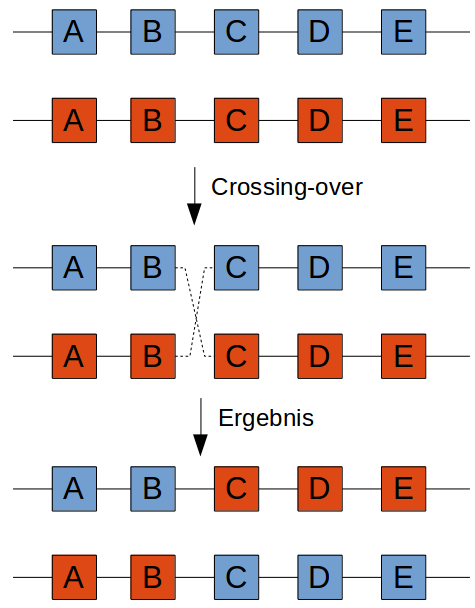
\includegraphics[width=0.5\textwidth]{lectures/V2/pix/crossing_over_b.png}
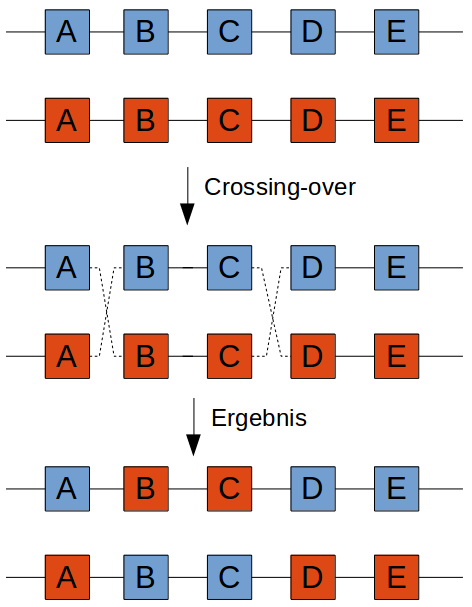
\includegraphics[width=0.5\textwidth]{lectures/V2/pix/crossing_over_c.png}

\subsubsection{Aufgabe 2}
Gen: ABO\footnote{\url{http://www.snpedia.com/index.php/ABO}}
rs8176719\footnote{\url{http://www.snpedia.com/index.php/rs8176747}}:
\begin{itemize}
	\item (-;-): likely to be of blood type O
	\item (-;G): most likely to be of blood type A or B
	\item (G;G): most likely to be of blood type A, B or AB 
\end{itemize}

rs8176747\footnote{\url{http://www.snpedia.com/index.php/rs8176747}}:
\begin{itemize}
	\item G führt zu Blutgruppe A, C zu Blutgruppe B
\end{itemize}

rs8176750\footnote{\url{http://www.snpedia.com/index.php/rs8176750}}: definiert Untergruppe von A
\begin{itemize}
	\item (-;C): A1
	\item (-;-): A2
\end{itemize}

Kombinationsmöglichkeiten:
\begin{itemize}
	\item praktisch durch Allele vorgegeben: $3 \cdot 2 \cdot 2 = 12$\footnote{\url{https://sites.google.com/site/abobloodgroup/14.aboalleles\%28oalleles\%29}}
	\item theoretisch: $5^3=125$
	\item \underline{Musterlösung:} 3 SNPs auf einem Allel $\rightarrow$ 8 Kombinationen; 2 Allele: 36 Möglichkeiten
\end{itemize}

A und B kodominant, Faktor 0 rezessiv

\subsubsection{Aufgabe 3}

\textbf{a.)}

\textbf{b.)}

\textbf{c.)}

\subsubsection{Aufgabe 4}

\textbf{a.)}\\
\underline{rezessiv:}\footnote{\url{https://de.wikipedia.org/wiki/Rezessiv}} bedeutet in der Genetik „zurücktretend“ oder auch „nicht in Erscheinung tretend“

\underline{dominant:}\footnote{\url{https://de.wikipedia.org/wiki/Dominanz_(Genetik)}} ein dominantes Allel setzt sich in der Merkmalsausprägung gegenüber einem rezessiven Allel durch

\underline{Penetranz:}\footnote{\url{https://de.wikipedia.org/wiki/Penetranz_(Genetik)}} prozentuale Wahrscheinlichkeit, mit der ein bestimmter Genotyp zur Ausbildung des zugehörigen Phänotyps führt
\\\\
\textbf{b.)}\\
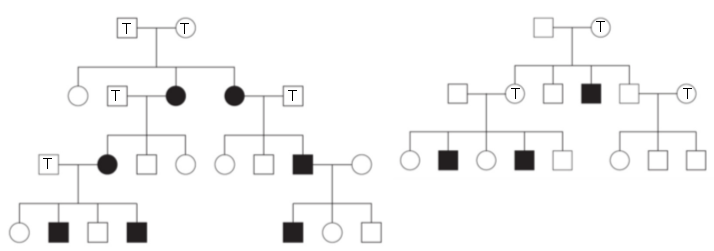
\includegraphics[width=1\textwidth]{lectures/V2/pix/stammbaeume1.png}
\newpage
\underline{aus Musterlösung:}\\
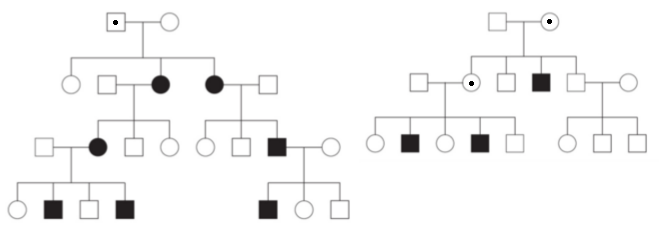
\includegraphics[width=1\textwidth]{lectures/V2/pix/standard_solution.png}
\\\\
\textbf{c.)}\\
\underline{links:} autosomal rezessiv, \underline{aus Musterlösung:} autosomal dominat mit reduzierter Penetranz, weil:
\begin{itemize}
	\item beide Geschlechter betroffen
	\item in jeder Generation
	\item etwa die Hälfte der Kinder betroffen
\end{itemize}

\underline{rechts:} genosomal rezessiv, auf einem X-Chromosom der Mutter\\